\vspace{-3mm}
\section{}
%%------------------------------------------------------------------------------------------
%                                   Cose Reference
%%------------------------------------------------------------------------------------------
\vspace{-4mm}
\subsection*{CODE}
\vspace{-3mm}
Experimnet 3의 동일한 network에서 CSMA 를위한 condition을 추가한다. 뿐만 아니라 조금더 복잡한 네트워크 환경을 simulation 해주기 위해서 inference range의 설정을 통해서 host a와 host b 사이에서 전송을 할 수 없지만 이에 따른 간섭의 영향을 추가한다.
사용하는 csma protocol에 ack응답을 추가해주어 신뢰성을 높인 네트워크를 simulation 한다.
\vspace{-3mm}
\subsubsection*{Experiment04.ini}
    \vspace{-2mm}
    \begin{listing}[h!]
    \inputminted[framerule = 1pt,framesep = 2mm , frame = lines, fontsize=\footnotesize ]{c}{./code/week12/Experiment_04/ini.cpp}
    \vspace{-3mm}
    \caption{\footnotesize Expeirment 03's ini file, using csma/ca as MAC with ACK}
    \end{listing}
    \vspace{-6mm} 
%%%%%%%%%%%%%%%%%%%%%%%%%%%%%%%%%%%%%%%%%%%%%%%%%%%%%%%%%%%%%%%%%%%%%%%%%%%%%%%%%%%%%%%%%%%%
%%------------------------------------------------------------------------------------------
%           simulation results -> you tube 링크 + 스크린샷 2장 + 내용에 대한 설명
%%------------------------------------------------------------------------------------------
\subsection*{SIMULATION RESULTS}
    simulation 전체의 영상은 아래 링크를 클릭하여 확인할 수 있다.     
    \vspace{-10mm}
        \begin{center}
            \item \href{https://www.youtube.com/watch?v=WlI24BkZjFs&ab_channel=anamnesis}
        	{Youtube link of Week12 Experiment 04 Simulation Results Screenshot Video}
        \end{center}
    \vspace{-6mm}
    % 사진 1 2개는 넣어 주자
         
\vspace{-3mm}
    \subsubsection*{Physical Layer Modelling  }
    \vspace{-2mm}
    ini 에서 가능한 무선 통신 연결거리를 500m, 1Mbps의 속도로 데이터가 전송이되고, ned 에서 Host A 와 Host B의 간격을 450m 로 설정해주어 직접 통신이 가능하도록 설정해 주었다. 
\vspace{-1mm}
    \subsubsection*{Simulation Scenario }
    \vspace{-2mm}
    앞선 experiment 1,2의 MAC  protocol들은 채널상에 올라온 패킷들을 즉시 전송하여 collision이 구조적으로 높게 발생하였다. 
    CSMA /CA는 다른 노드들의 전송상태를 채크함으로서 충돌을 회피한다. 여기에 ACK 을 사용하여 다른 노드들에게 채널이 비어있음을 알린다.
    Host A 에서 임의의 간격으로 UDP packet을 생성해주고, 생성된 packet은 IPv4 를 통해서네트워크 later로 이동한다. 이때 네트워크 layer에서 packet은 전송 대기열이 진행하는 simulation처럼 없으면 바로 전송이 이뤄진다. 이후 Host A 에서 Host B로 바로 모든 packet이 전송된다. 
\section*{Discussion}
\vspace{-3mm}
실험 2,3 그리고 4를 진행하면서 네트워크의 변화는 다음과 같다. 
\vspace{-3mm}
    \subsubsection*{EX02 $\rightarrow$ EX03}
\vspace{-2mm}
Routing host를 추가하고 Host A와 Host B사이의 통신이 Host R1을 통해서 이루어지게 된다.
Hidden Node Problem으로, 전송되는 UDP packet을 확인해 보았을때 NIC 에서 각 NODE들은 언제나 수신하거나 송신할 수 있지만 동시에 진행이 되지 못하기 떄문에 실질적으로 전송되는 PACKET의 수는 실험 3에서 실험 2와 비교해 보았을때 절반정도만 전송이 되는 결과를 확인할 수 있었다. 
\vspace{-3mm}
    \subsubsection*{EX03 $\rightarrow$ EX04}
\vspace{-2mm}
실험 3의 network 에서 ACK을 사용하는 CSMA / CA를 MAC으로 사용한다. 추가로 ACK의 사용여부에 따른 차이를 확인하기 위해서 ini 파일에서 \mintinline{c}{host*.wlan[0].mac.useAck = false}로 설정해준 일반 CSMA의 실험을 진행해 주어 결과를 비교해 보았다. Figure 6 (a)에서 UDP-Packet 0 가 전송되는 과정을 보면, Host R1 에서 Host B로 back off timer가 지난후 바로 전송이 이루어짐을 확인할 수 있다. 이 과정에서의 소요시간을 실험 2 와 비교해 보면 대략적으로 7배 빠른 CSMA 의 이점을 확인할 수 있다. 

Figure 6 (b) 에서는 추가적으로 ACK을 사용함으로서, Host R1 에서 Host B 로  UDP-Packet 0을 전송할때 확산시키는 CsmaAck을 수신받아야 UDP packet을 전송하는 과정으로 실험3에서 일정시간 후 전송에서 변화된점을 확인할 수 있다. 이를 통해서 ACK이 없는경우에 비해 손실된 packet이 거의 없이 안정적으로 데이터를 전송할 수 있지만, 만일 네트워크가 혼잡한 경우 collision에 따라서 ACK의 수신에 따른 delay가 심화될 수 있는 단점 또한 확인할 수 있다.\\
\begin{figure}[h!]
\centering
\subfloat[Experiment04 csma ]{
    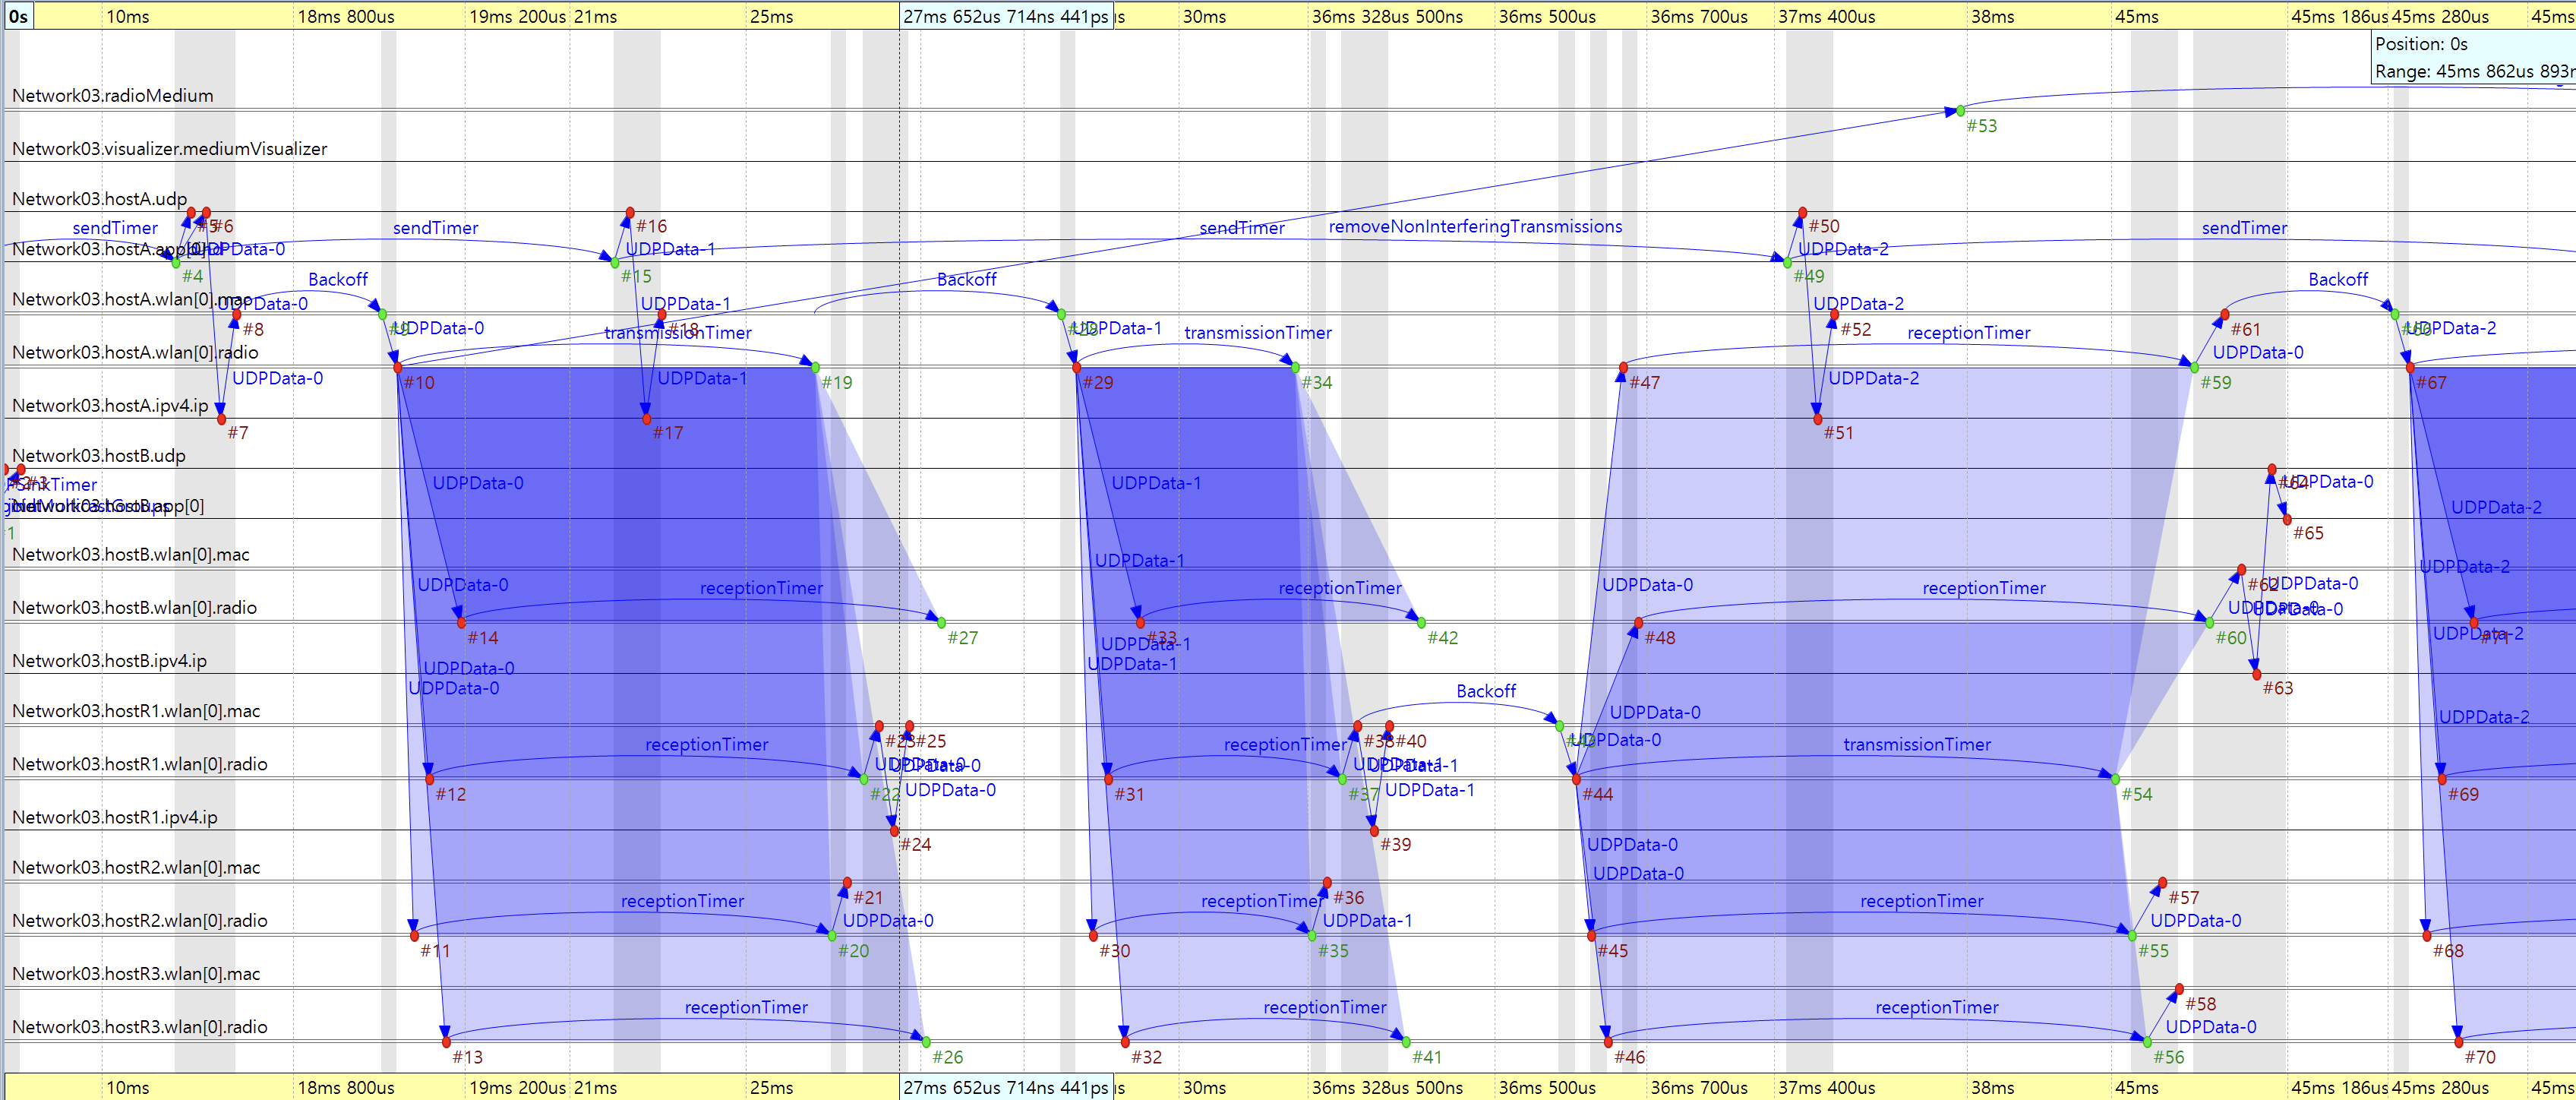
\includegraphics[width=0.9\textwidth]{image/week12/5-1.png}
}\hspace{3mm}
\subfloat[Experiment-4 csma / ca]{
    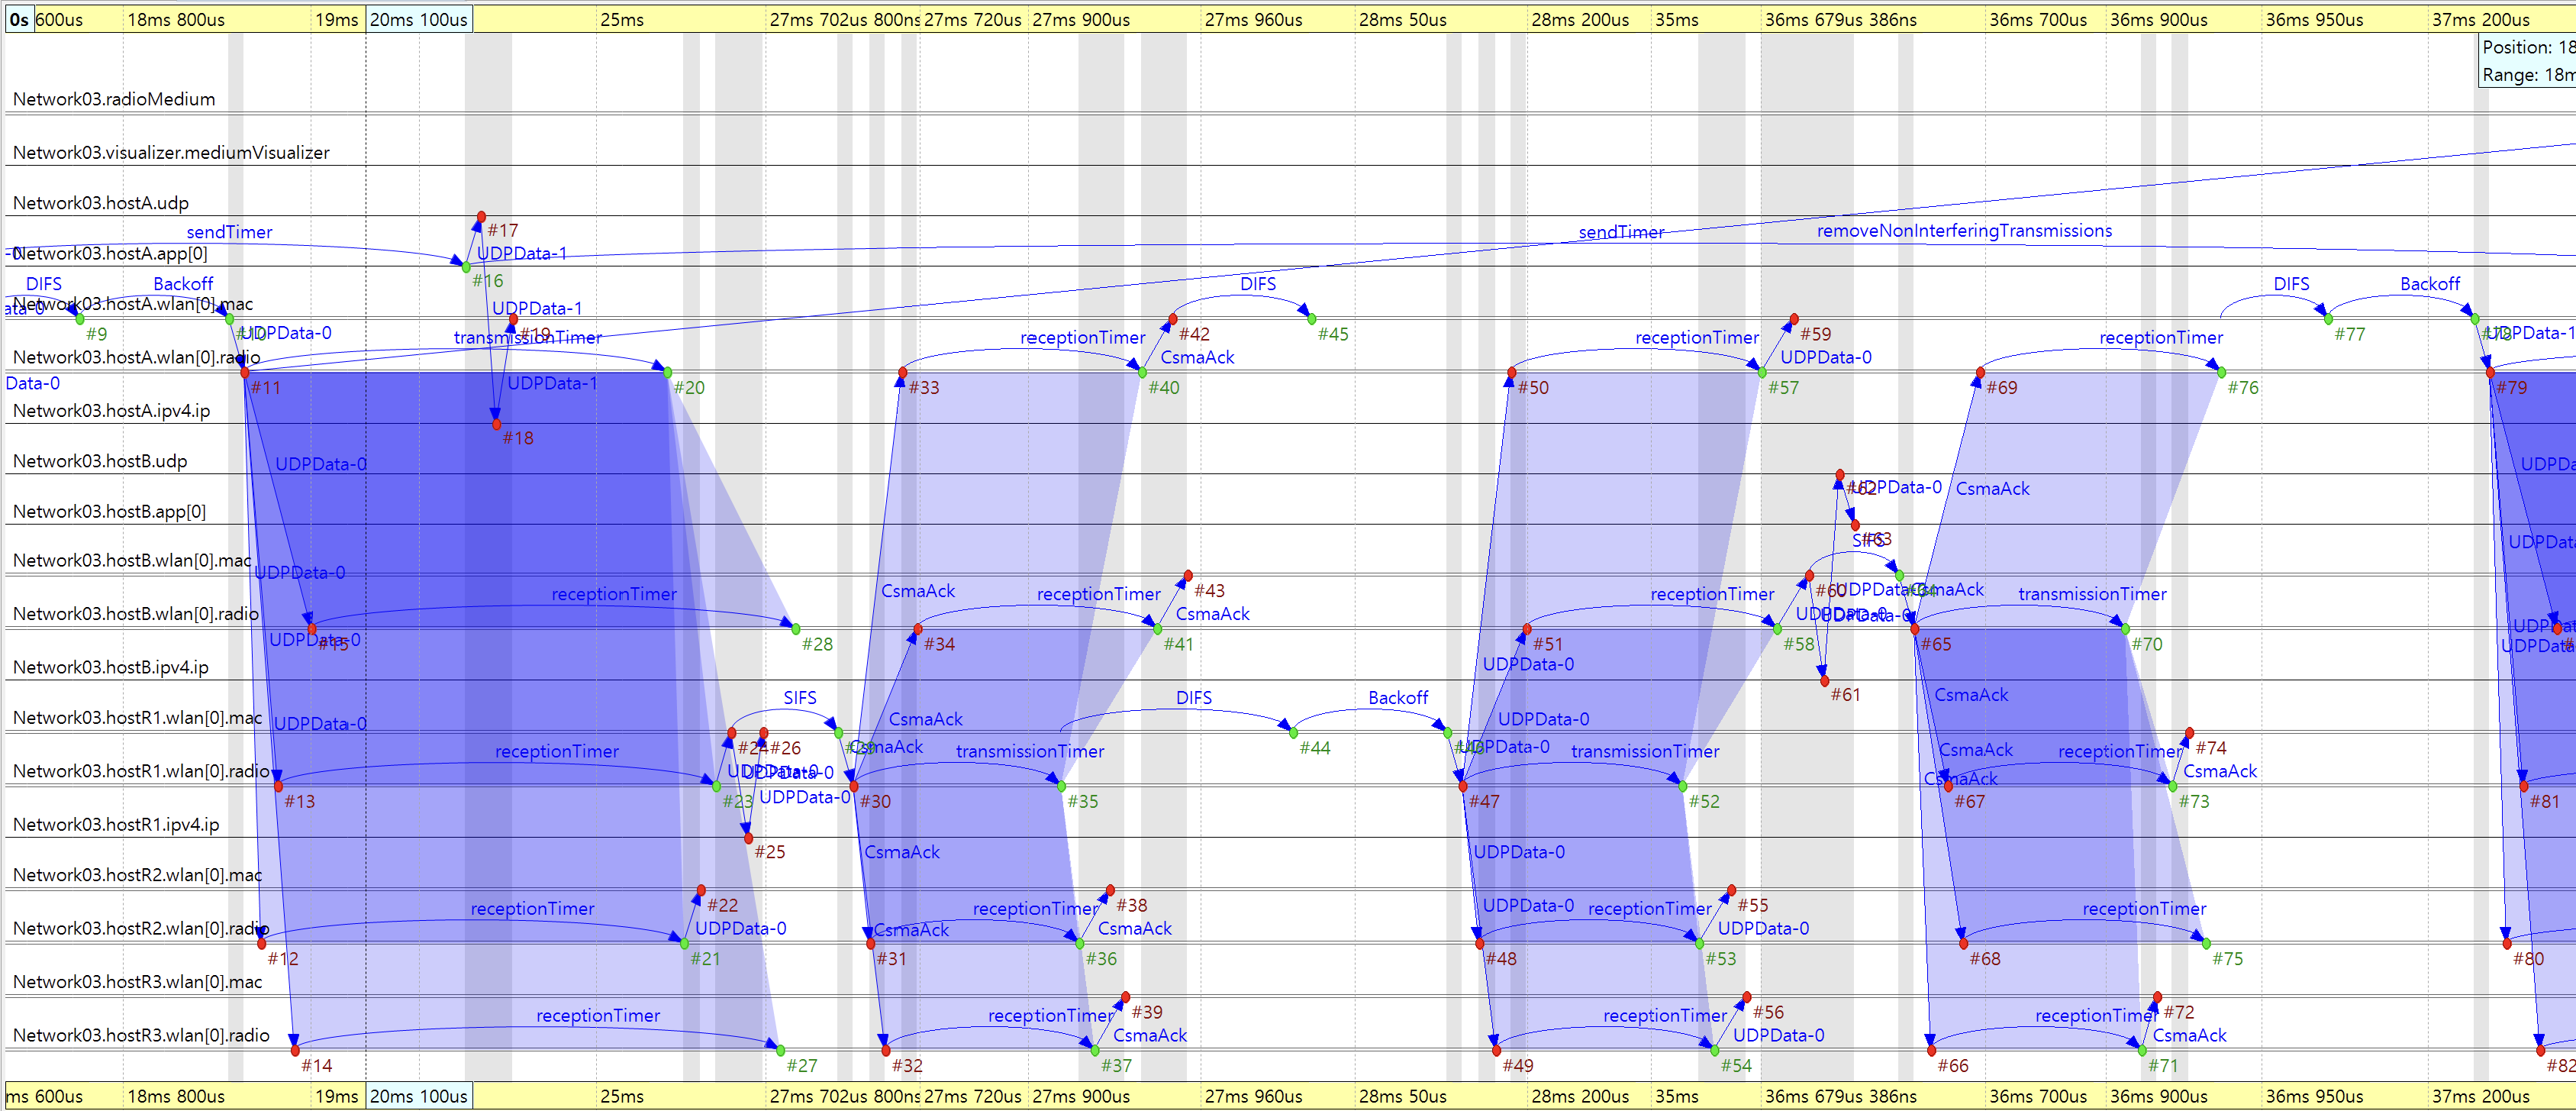
\includegraphics[width=0.9\textwidth]{image/week12/5-2.png}
}
\end{figure}

\clearpage